%!TEX root = ../main.tex
\chapter{Implementation and Evaluation}

%Damien's words not mine
For clarity, we present the implementation and evaluation together and split the presentation by the natural split in the code which is the server and application.

\section{Application}
\subsection{Android}
Android has been chosen for this application due to the large success and market hold of the operating system.
Primarily I will be aiming to support Android versions down to API level 16 (Jelly Bean 4.1).
This decision has been made as appendix \ref{appendix:sdkmarketshare} shows that by supporting this far back, the application will be compatible with over 95\% of current phones. 
Older versions than this will not be targeted, as development and testing time is limited and it would mean that many features would have to be limited due to lacking functionality within these older versions.

\subsection{Google Cloud Messaging}
The app will be responsible for relaying information between the parent and child clients in a reliable and timely manner.
In Android, this can be achieved using push notifications relayed through the Google Cloud Messaging (GCM) service.
GCM can be utilized to send messages to an Android device, but is largely unreliable \citep{gcmreliability} and therefore should only be used for notifications, rather than the transmission of data.
The service requires that the server registers with the GCM to retrieve an API key and that the user device registers to retrieve a GCM registration ID \citep{gcm}. 
When a user registers with the artefact server, the registration ID is stored wtihin the database to be used to send notifcations.
When a particular action is performed on an account in the API, the server will check if that user has an attached account - i.e. either a Parent monitoring a Child or vice versa.
Then, the server sends the message and the target GCM registration ID to the GCM system which passes on the message.

Within the application, a listener service has been implemented to be triggered upon the receipt of a GCM message that will create a push notification with the message sent by the server.
Examples of the push notification messages can be seen in appendix \ref{appendix:pushnotifications}.

\section{Server}
\subsection{Representational State Transfer (REST)}
To structure the server's web services, I have chosen to use a REST architecture style.
REST involves dividing the web services into specific objects which can be accessed through sending a request to that object's URL, this is called an `endpoint' or a `URI'.
These endpoints are then connected to via different HTTP methods, of which the following are used:
\begin{description}[align=left]
	\item [GET] Retrieves an item or list of items.
	\item [POST] Creates a new item.
	\item [PUT] Updates an existing item or list of items.
	\item [DELETE] Deletes an item.
\end{description}
For example, if someone wanted to retrieve all users of a REST service, they could send a GET request to the `/users/' endpoint. 
If, however, they wanted to retrieve a specific user, they would send a GET request to `/users/$x$/' where $x$ is the user's ID.
And finally, sending a POST request to `/users/$x$/quests/' would create a a new quest for user $x$.

Collectively, these request methods and endpoints will form the basis for all communication with the server. 
A full plan for the endpoints of the server artefact can be seen in appendix \ref{appendix:endpoints} and examples of requests in \ref{appendix:requests}.

\subsection{Flask}
For the server-side implementation, I will need tools that allow me to easily create a web service API and provide controlled access to functionality over the web.
For this task, I chose to use Flask as it is well established within the Python community and is relatively easy to set up and maintain. 
Flask is suitable for both quick prototyping of web-services and reliable deployment/hosting of the functionality over the internet.

By utilizing Flask, I was able to easily translate a user's web request into a method call, with relevant parameters, using the following code:
\lstinputlisting[language=python]{codesnippets/getrewards.py}
This short code snipped shows the method used to return all rewards in the reward shop for a user.
This method is activated upon sending a GET request to the endpoint such as `server\_host\_name:5000/api/user/1/rewards/', and will return the rewards for the first user in JSON format, provided the attached authentication details match that user. 

\subsubsection{JSON vs. XML}
In order to communicate to the servers web services, I will need to decide upon a message format. 
REST is capable of using both XML and JSON to communicate over the web and neither is a more reliable form of transferring data, but there are minor advantages/disadvantages to each.

%TODO: Source the shit out of this
JSON is better supported by numerous libraries and or



\subsection{SQLite}
\subsubsection{Object-Relational Mapper}
I chose to use a pre-built Object Relational Mapping library to interface with the database, rather than crafting particular queries on an ad hoc basis. 
This was primarily for more ease-of-use purposes than any performance reasons. 
I considered a variety of options for which library to use, initially deciding upon SugarORM due to its very quick learning curve and low use of boilerplate syntax. 

%SQLAlchemy

Implementing an ORM also allows me to more easily protect the application against malicious SQL injection attacks as both GreenDAO and SQLAlchemy provide sufficient protection against this. 


%Reconsider this writing



\subsection{Server Rewrite}
The plan was then to send the quests to the parent phone using Google Cloud Messaging (GCM) and have them send back which quests were completed.
However, GCM was not suitable for moving the quests reliably and I found that it was too likely that information would be lost or become out of sync between parent and child devices.

Therefore, I decided to push most of the data and functionality to the server-side and have the app interact with the server to perform actions.
I still chose to use GCM for communicating from the server to a client in order to push notifications when tasks are confirmed or completed.





Separating child and parent users was a mistake.

\section{Game Design}
\subsection{Rewards}
The rate at which these rewards are earned must be examined to ensure they still feel rewarding throughout. 
For example, if a quest returns 100 XP points and you require 300 XP to level up from level 1 to 2, this only requires you to complete three quests to level up, meaning these three quests feel rewarding as each quest is offering 1/3rd of a level.
However, the XP if quests still offer 100 XP and you require 6000 XP to level up from level 30 to 31, the reward from the same quest is now worth 1/60th of a level, despite being the same difficulty to the user.
Therefore, some scaling of the rewards is required in the app to allow XP rewards to scale suitably with the XP required to level.
This scaling is referred to as `increasing cost' \citep{1_anderson_2016}.
Anderson also shows that it is important to determine reasonable caps for numerical relationships in video-games, to stop the increasing cost becoming out of proportion.

\cite{1_anderson_2016} poses that a useful pattern for these kinds of relationships is a classic triangular pattern, in which the first level requires 1 XP to level up, the second level requires 3 XP, the third requires 6. To allow for more meaningful numbers to the user, I have multiplied the results of the formula by 100.

\begin{equation} \label{eq:xprequiredfornextlevel}
	T_n= \frac{n(n+1)}{2} \times 100
\end{equation}

Initially, the scaling formula for XP rewards involved using 60XP as a base reward for a medium difficulty quest, then using the player's current level, it would derive a multiplier that would be used to scale the XP reward.

\begin{equation} \label{eq:xpgainedlinear}
	\textrm{XP Gained} = 60 \times \frac{(n - 1) \times k}{100} + 1
\end{equation}

Where k can be adjusted to specify the strength of the multiplier against the XP rewards, so that if k = 10, a character at level 31 would have a 3x multiplier on quests, meaning the same quest that gave them 60XP at level 1, now gives them 180XP.
However, when modelling this equation, the number of quests completed quickly becomes out of hand. 
At level 1, the player must complete 2 medium quests to level up - a reasonable starting point.
However by level 25 the player must complete 22 quests to level up and by level 99 (One before the level cap) the player must complete an extraordinary 84 medium difficulty quests to level up.

Therefore, triangular numbers can also be useful for calculating the XP gained per quest. By adjusting the triangular numbers formula somewhat, I found a suitable middle ground which still gives the new user the feeling of progressing quickly, but the rate of quests per level quickly slows down to a limit of approximately 10 quests per level by level 100.
This will ensure that the player will still feel like they are progressing at a reasonable speed throughout.

\begin{equation} \label{eq:xpgainedtriangular}
	\textrm{XP Gained} = \frac{(n+2)(n+3)}{2} \times 10
\end{equation}

\begin{center}
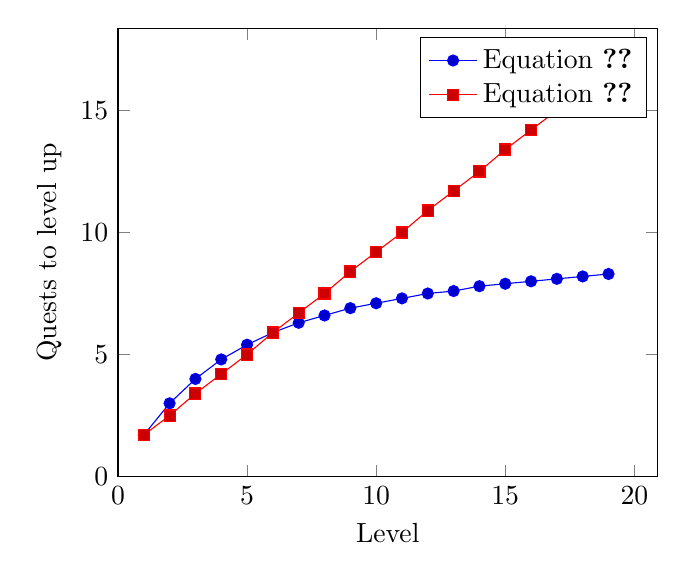
\begin{tikzpicture}
	\begin{axis}[
		xlabel=Level,
		ylabel=Quests to level up,
		xmin=0,
		ymin=0,
	]
		\addplot coordinates {
			(1, 1.7)
			(2, 3)
			(3, 4)
			(4, 4.8)
			(5, 5.4)
			(6, 5.9)
			(7, 6.3)
			(8, 6.6)
			(9, 6.9)
			(10,7.1)
			(11,7.3)
			(12,7.5)
			(13,7.6)
			(14,7.8)
			(15,7.9)
			(16,8)
			(17,8.1)
			(18,8.2)
			(19,8.3)
		};
		\addlegendentry{Equation \ref{eq:xpgainedtriangular}}
		\addplot coordinates{
			(1, 1.7)
			(2, 2.5)
			(3, 3.4)
			(4, 4.2)
			(5, 5)
			(6, 5.9)
			(7, 6.7)
			(8, 7.5)
			(9, 8.4)
			(10, 9.2)
			(11, 10)
			(12, 10.9)
			(13, 11.7)
			(14, 12.5)
			(15, 13.4)
			(16, 14.2)
			(17, 15)
			(18, 15.9)
			(19, 16.7)
		};
		\addlegendentry{Equation \ref{eq:xpgainedlinear}}
	\end{axis}
\end{tikzpicture}
\end{center}

\subsection{Gold Rewards}
A key goal of the project is achieving long term motivation for children, and to avoid the non-continuous effects mentioned by \cite{deci2001extrinsic} in chapter 2 research.
In order to achieve this goal, I implemented two key elements to the rewards earned from a quest.

Firstly, in order to discourage Child users from delaying performing a task, I implemented a system that gradually diminishes the maximum achievable gold reward for a quest over time. 
In this system, a quest is added with an expiry date value, which defaults to one week from the quest creation date.
At around halfway through the time available to complete the task, the reward from the quest will begin to reduce at a steady rate for the remaining time.
Eventually, if the task remains incomplete until the expiry date, the gold reward drops to zero, the quest expires and the quest is removed from their tasks.


Secondly, 

\begin{equation} \label{eq:openloopreward}
	yk = ax_k + by_{k-1} + cy_{k-2}lc
\end{equation}




\section{Testing}
Unfortunately, when developing a REST API, it is difficult to manually write and send the request to the API to test it.
Programs and scripts exist to ease the process somewhat, but I found the easiest way to be automating the requests entirely. 
As a main principle of REST is to plan out the specific endpoints that can be messaged, it becomes rather simple to plan out tests in the form of sending an example of a valid and invalid request of each request type to each endpoint.
For example, the endpoint of `/api/users/<userId>/' allows two request types, GET and PUT, which generates four test cases.
\begin{itemize}
	\item{Valid GET}
	\item{Invalid GET}
	\item{Valid PUT}
	\item{Invalid PUT}
\end{itemize}  
%TODO: Research what test generation this is

However, this raises issues when considering that a request could be invalid for multiple reasons, and simply testing for invalid/valid may not reach adequate code coverage.
An example of this could be that a PUT request may be invalid due to an email address already existing within the database or because they have not included a valid did not include any new data about the user, which are two separate sections of the code that arguably each require their own tests.
This issue is highlighted by \cite{4597151}, who states that testing a program tells us `little about its quality', arguing that the quality of a test case far outweighs sheer quantity of tests.
Because of this, it must be analysed whether or not the test cases achieve sufficient code coverage, rather than just relying on the entry points into the software.
Luckily, the python package `coverage.py' allows for simple analysis of unit tests to determine the current code coverage for tests, which will provide a higher rate of confidence.

\subsection{Test-Driven Development}
In the creation of a REST API, it is much easier to develop a test plan due to the clearly laid out workflow of the user. From the server's point of view, there are only a handful of requests that a user can make, and only a handful of tests for those requests. Before writing each endpoint of the server, I 

\subsection{Unit Testing} 
As a part of Test-Driven Development, unit testing is a integral part of the development process.

%Server

For the server, I will an extension library of Flask called Flask-Testing, which streamlined the process of writing and running unit tests.
Flask-Testing allows you to create a new instance of your Flask application with a separate configuration file which can be changed to make the app connect to a different MySQL database file - in this case it connected to a freshly generated and empty test database.
Then, as each separate test case is run, I used the library to delete the test database and regenerate it to ensure that previous unit tests would not interfere with new tests.

For example, the following code is a simple test that creates a child user on the server, then attempts to get the user details from the server without authorizing itself first. 
The test will pass if the server correctly rejects the request with a `401: Not Authorized' error or fail otherwise.
\lstinputlisting[language=python]{codesnippets/serverunittest.py}

\subsection{Integration Testing}
Integration testing encompasses tests that specifically test that the various parts of the project work together correctly.
For example, in this project, integration tests would test that the server and mobile app are able to correctly function together, by ensuring that the app can correctly send requests and that the server receives those requests as they were sent.


\subsection{Black Box Testing}
Black box testing describes the testing of software without using explicit knowledge of the code.
Essentially, it is testing by using that the usage of the application is correct

\subsection{White Box Testing}


\subsection{Regression Testing}
Regression testing is the practice of retesting the previously tested parts of the software to ensure that they are still performing correctly after a change elsewhere in the code, it can also be used to describe the process of testing previously detected and fixed bugs to determine that they have not reappeared.
This is made significantly easier by the implementation of strong automated unit tests, which allow me to quickly retest the majority of the code by rerunning the test suite.
I also intend to follow a common development practice where a unit test is added for each defect that is found within the code, a new unit test is added to detect the presence of that bug specifically. 
This will allow me to easily spot any recurrences of legacy bugs that would otherwise go unnoticed.
